\documentclass{article}
\usepackage{fancyhdr}
\pagestyle{fancy}
\fancyfoot{}
\fancyfoot[C]{\thepage}
\rhead{Yarosevich - 1064712}
\usepackage{setspace}
\usepackage{siunitx} % Provides the \SI{}{} and \si{} command for typesetting SI units
\usepackage{graphicx} % Required for the inclusion of images
\usepackage{amsmath} % Required for some math elements 
\usepackage[export]{adjustbox} % loads also graphicx
\usepackage{listings}
\usepackage{setspace}
\usepackage{matlab-prettifier}
\usepackage{float}
\usepackage[most]{tcolorbox}
\usepackage{amsfonts}
\usepackage{color}
\usepackage{physics}
\usepackage{titlesec}
\usepackage{caption}
\usepackage{subcaption}
\usepackage{python}
\usepackage{placeins}
\usepackage{bm}
\usepackage{esvect}
\newcommand{\uveci}{{\bm{\hat{\textnormal{\bfseries\i}}}}}
\newcommand{\uvecj}{{\bm{\hat{\textnormal{\bfseries\j}}}}}
\DeclareRobustCommand{\uvec}[1]{{%
  \ifcsname uvec#1\endcsname
     \csname uvec#1\endcsname
   \else
    \bm{\hat{\mathbf{#1}}}%
   \fi
}}


\newcommand{\R}{\mathbb{R}}

\usepackage{xcolor}

\DeclareCaptionFont{white}{\color{white}}
\DeclareCaptionFormat{listing}{%
  \parbox{\textwidth}{\colorbox{gray}{\parbox{\textwidth}{#1#2#3}}\vskip-4pt}}
\captionsetup[lstlisting]{format=listing,labelfont=white,textfont=white}
\lstset{frame=lrb,xleftmargin=\fboxsep,xrightmargin=-\fboxsep}
\titleformat{\section}[runin]
  {\normalfont\Large\bfseries}{\thesection}{1em}{}
\titleformat{\subsection}[runin]
  {\normalfont\large\bfseries}{\thesubsection}{1em}{}


\setlength\parindent{0pt} % Removes all indentation from paragraphs

\renewcommand{\labelenumi}{\alph{enumi}.} % Make numbering in the enumerate environment by letter rather than number (e.g. section 6)

%\usepackage{times} % Uncomment to use the Times New Roman font

%----------------------------------------------------------------------------------------
%	DOCUMENT INFORMATION
%----------------------------------------------------------------------------------------

\title{AMATH 522: Homework 1 \\Due October, 9 2019 \\ ID: 1064712} % Title

\author{Trent \textsc{Yarosevich}} % Author name

\date{\today} % Date for the report

\begin{document}
\maketitle % Insert the title, author and date
\setlength\parindent{1cm}

\begin{center}
\begin{tabular}{l r}
%Date Performed: December 1, 2017 \\ % Date the experiment was performed
Instructor: Professor Eric Shea-Brown % Instructor/supervisor
\end{tabular}
\end{center}
\doublespacing
% If you wish to include an abstract, uncomment the lines below
% \begin{abstract}
% Abstract text
% \end{abstract}

%----------------------------------------------------------------------------------------
%	SECTION 1
%----------------------------------------------------------------------------------------
\section*{\textbf{(II)}}
Below are the plots of the the log of the total population over time, as well as the fraction of each age group relative to total population over time. 
\begin{center}
    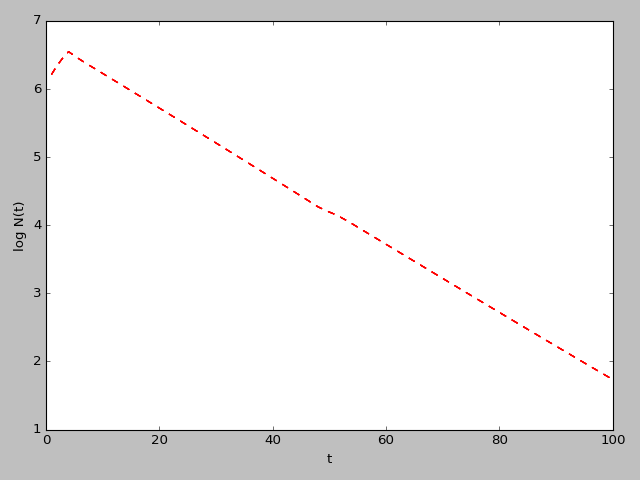
\includegraphics[scale = .3]{part1_log_plot.png}
    %\captionof{figure}{D}
    %\label{fig: D}
    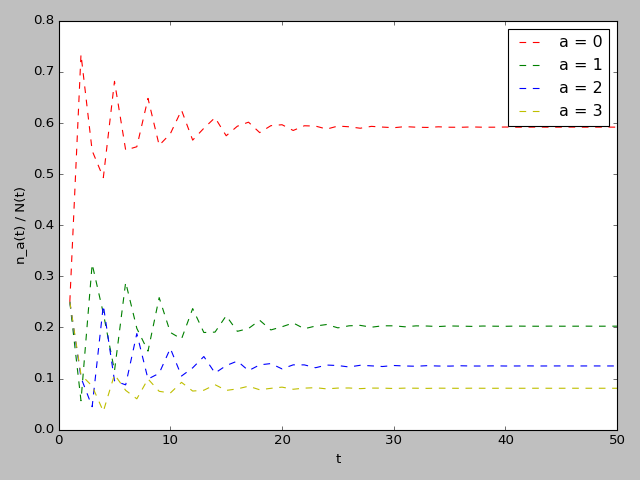
\includegraphics[scale = .3]{part1_frac_plot.png}
    %\captionof{figure}{D}
    %\label{fig: D}
\end{center}




By "write down the Euler-Lotka formula for this example" I assume this means the specific formula to update the population and not the general equation. If we have
\begin{gather}
 A=
  \begin{bmatrix}
   0 &
   1 &
   5 &
   .5 \\
   .5 &
   0 &
   0 &
   0 \\
   0 &
   .9 &
   0 &
   0 \\
   0 &
   0 &
   .95 &
   0
   \end{bmatrix}
 \end{gather}
then the update equation is $n(t+1) = An(t)$. The estimated growth rate $\lambda$ from fitting a polynomial to the first graph is $\lambda = 1.462571$ and the numerically calculated value from the $A$ matrix is $\lambda = 1.46237$, so clearly they are very close - the difference is probably explained by the error in the curve fitting. \\
\\
Here is the code used for this section:
\lstset{language=Python}
\lstset{frame=lines}
\lstset{label={lst:code_direct}}
\lstset{basicstyle=\footnotesize}
\begin{lstlisting}
#%% Part II
import numpy as np
import matplotlib.pyplot as plt

# Declared col. vector of initial populations
n_0 = np.array([[100, 100, 100, 100]])

# Vector of fecundity values, intermediate array
# for survival probabilities
fecun = np.array([0, 1, 5, .5])
p_i = np.diag([.5, .9, .95, 0])

# Adding fecundity onto the survival array and
#removing excess row.
A = np.row_stack([fecun,p_i])
A = np.delete(A, 4, 0)

t_max = 50
t_mesh = np.arange(1, t_max +1)

# Declaring population array and inputting initial condition.
n_t = np.zeros((4, t_max))
n_t[:, 0] = n_0

# Time-steps through the t-mesh starting at t=1
for t in range(1, t_max):
    n_t[:, t] = np.dot(A, n_t[:, t-1])

# Calculates the total population size, i.e.
# the sum of each age-population. Then declares
# an array representing the fraction of each age
# population of the total population at time t.
N_t = np.sum(n_t, 0)
w_t = n_t / N_t


plt.figure(1)
plt.plot(t_mesh, np.log(N_t), 'r--')
plt.xlabel('t')
plt.ylabel('log N(t)')

plt.figure(2)
plt.plot(t_mesh, w_t[0,:], 'r--', label = 'a = 0')
plt.plot(t_mesh, w_t[1,:], 'g--', label = 'a = 1')
plt.plot(t_mesh, w_t[2,:], 'b--', label = 'a = 2')
plt.plot(t_mesh, w_t[3,:], 'y--', label = 'a = 3')
plt.xlabel('t')
plt.ylabel('n_a(t) / N(t)')
plt.legend()

plt.show()

# Polyfits a 1st degree polynomial to the data and
# declares the estimate of lambda.
poly_coeff = np.polyfit(t_mesh, np.log(N_t),1)
lambda_est = np.exp(poly_coeff[0])

# Declares a variable holding the maximum mathematically
# calculated eigenvalue of A.
lambda_dom = np.amax(np.linalg.eigvals(A))
\end{lstlisting}
\section*{\textbf{(II)}}
\subsection*{\textbf{(a)}}
If we iterate using eigenvalues we have the population that reaches adulthood from the initial population of newborns given by $n_3(3)$ since it takes three time-steps for each adolescent population to potentially advance to adulthood. This can be written as $n_3(3) = c_2\lambda_2(c_0\lambda_0(c_1\lambda_1n_0(0)))$. The constants $c_i$ here are arbitrary and $c_i\lambda_i = p_i$, thus $n_3(t)$ in terms of an initial population of newborns can be written as $p_0p_1p_2n_0(0)$ and it is self-evident that the particular values of the coefficients do not matter so long as their product is consistent, in this case $0.0722$.
\subsection*{\textbf{(b)}}
The projection matrix is constructed in the code below.
\subsection*{\textbf{(c)}}
The dominant eigenvalue as calculated in the code below is $\lambda = 0.9517$
\subsection*{\textbf{(d)}}
Elasticity matrix is computed in the code. The elasticity for the fecundity values decreases very slightly as we move up the population stages. This makes sense perhaps because later fecundity values apply to older populations, which are inevitably going to be smaller. I would speculate that since the survival rate of adults is very high, this falloff is very slow.\\
\\
The elasticity for survival probability falls off quite a bit faster, and this makes a lot of sense since a younger animal surviving means quite a few more years to reproduce, whereas when an individual in, say, the 50th age group dies, they are only missing a single reproduction opportunity. This implies that, in regard to management plans, it would be ideal to find out if there might be a way to target the survival of younger individuals.\\
\\
Code for part III:
\begin{lstlisting}
#%% Part III
import numpy as np
import matplotlib.pyplot as plt

# b.) and c.)
#Constructing A matrix and inputing values
fecun_vec = .24 * np.ones(50)
fecun_vec[0:3] = 0
surv_mat = np.diag(.952 * np.ones(50))
surv_mat[0, 0] = 1
surv_mat[1,1,] = 1
surv_mat[2,2] = .0722

A = np.row_stack([fecun_vec,surv_mat])
A = np.delete(A, 50, 0)

# Setting up discrete time values and associated
# population value array with the n_0 values.
t_max = 100
t_mesh = np.arange(1, t_max + 1)
n_0 = 10 * np.ones(50)
n_t = np.zeros((50, t_max))
n_t[:,0] = n_0

# Iterating through the time steps.
for t in range(1, t_max):
    n_t[:, t] = np.dot(A, n_t[:, t-1])

# Total popluation for each time step.
N_t = np.sum(n_t, 0)
# plt.figure(3)
# plt.plot(t_mesh, np.log(N_t), 'r--')
# plt.xlabel('t')
# plt.ylabel('log N(t)')

# Estimating dominant eigenvalue and calculating directly.
poly_coeff = np.polyfit(t_mesh, np.log(N_t),1)
lambda_est = np.exp(poly_coeff[0])
lambda_dom = np.amax(np.linalg.eigvals(A))

#part d.)

# Storing the left and right eigenvectors, indexing the max
# eigenvalue. Taking the real values of the eigenvectors since the matrix
# A is power-positive.
w, vr = np.linalg.eig(A)
w2, vl = np.linalg.eig(A.T)
max_eig_index = np.argmax(w)
vr = vr[:,max_eig_index].real
vl = vl[:,max_eig_index].real

# Using an outer product of l/r eigenvectors and dividing
# by their dot product (scalar) to calculate sensitivity matrix.
# Weighting each entry to calculate the elasticity.
S_ij = (np.outer(vl, vr) / np.dot(vl,vr)).real
e_ij =  np.multiply( A / w[max_eig_index].real, S_ij)
\end{lstlisting}
\section*{\textbf{(IV)}}
All the relevant information for this part is in the code. My results were determined by simulating the population until its total size fell below one individual, since the decay is asymptotic and never reaches zero in a finite amount of time. My results were that a harvest of 5 juveniles per year was sustainable, and a harvest of 3 reproductive adults per year was sustainable. This is fairly sensible since the reproductive adults do the bulk of...reproducing. Here is the code:
\begin{lstlisting}
#%%
# Part IV For Juvinilles
import numpy as np
import matplotlib.pyplot as plt

# Declaring the Leslie Matrix
fecun = np.array([0, .0043, .1132, 0])
prob = np.array([[.9775, .9111, 0, 0], [0, .0736, .9534, 0], [0, 0, .0452, .9804]])
A = np.row_stack([fecun,prob])

# Declaring eigenvalue and eigenvectors in orer to find
# the dominant eigenvectors in order use the ratios therein
# to find a stable population distribution with a total of 250
# individuals.
w, v = np.linalg.eig(A)
max_eig_index = w.argmax()
eigvec_stable = v[:,max_eig_index]
eig_vec_sum = np.sum(eigvec_stable)
n_0 = (eigvec_stable / eig_vec_sum) * 250

t_max = 500
t_mesh = np.arange(1, t_max +1)

# Declaring population array and inputting initial condition. Putting
# a placeholder value in the total population array in order to start
# the while loop. Holder variable for the sustainable h value, as well
# as the initial population.
n_t = np.zeros((4, t_max))
n_t[:, 0] = n_0
n_t_start = n_t
N_t = np.sum(n_t, 0)
N_t[-1] = 2
h_sustainable = 0
h_list = np.zeros(4)

# Note the while loop condition is that there be greater than or
# equal to 1 individual, since presumable 99% of an Orca is not an Orca.
while N_t[-1] >= 1:
    h_sustainable = h_list[1]
    h_list[1] = h_list[1] + 1
    n_t = n_t_start
    for t in range(1, t_max):
        n_t[:, t] = np.dot(A, n_t[:, t - 1]) - h_list
        if n_t[1, t] < 0:
            n_t[1, t] = 0
    N_t = np.sum(n_t, 0)

#%%
# Part IV For reproductive adults
import numpy as np
import matplotlib.pyplot as plt

fecun = np.array([0, .0043, .1132, 0])
prob = np.array([[.9775, .9111, 0, 0], [0, .0736, .9534, 0], [0, 0, .0452, .9804]])
A = np.row_stack([fecun,prob])

w, v = np.linalg.eig(A)
max_eig_index = w.argmax()
eigvec_stable = v[:,max_eig_index]
eig_vec_sum = np.sum(eigvec_stable)
n_0 = (eigvec_stable / eig_vec_sum) * 250

t_max = 500
t_mesh = np.arange(1, t_max +1)

# Declaring population array and inputting initial condition.
n_t = np.zeros((4, t_max))
n_t[:, 0] = n_0
n_t_start = n_t
N_t = np.sum(n_t, 0)
N_t[-1] = 2
h_sustainable = 0
h_list = np.zeros(4)

while N_t[-1] >= 1:
    h_sustainable = h_list[2]
    h_list[2] = h_list[2] + 1
    n_t = n_t_start
    for t in range(1, t_max):
        n_t[:, t] = np.dot(A, n_t[:, t - 1]) - h_list
        if n_t[2, t] < 0:
            n_t[2, t] = 0
    N_t = np.sum(n_t, 0)
 \end{lstlisting}

 \section*{\textbf{(V)}}
 I took 301 and 481, and so insofar as matlab programming goes there wasn't anything new to me in this assignment. I decided to code it up in python, as I've been meaning to migrate in this direction as much as possible given its prevalence outside academia. As a result, I learned quite a bit about numpy syntax while working on this problem. I'd say the biggest two take aways for me were:\\
 \\
 1.) Numpy is, for the most part, agnostic in regard to column/row arrays. That is to say, if you utilize the correct functions and directly call operators like dot products or outer products, as opposed to casting arrays as matrices and using the * operator for example, then everything can simply remain a 'row' array. I put row in quotes since, so far as I understand it, 1xn array in numpy doesn't even have a second dimension unless cast as a matrix.\\
 \\
 2.) Pycharm supports code block separators just like matlab, which is nice. These are simply put in the code as a 'hashtag percent percent' (which I annoyingly cannot write out in sublime text because it provokes built-in environments) and then you can run blocks of code while working on a project, without creating lots of main functions or classes. As a sidenote to this, there is no super easy way to automatically wipe the variables when doing this like there is in matlab. If using the anaconda interpreter, however, the console will be ipython by default, and one can simply type percent reset -f (again stupid sublime text env) in the console at any time to clear the use declared variables. Very handy!

 \section*{\textbf{(VI)}}
 \subsection*{\textbf{(a)}}
 I read the paper "Microbes can help explain the evolution of host altruism" by Lewin-Epstein, Aharonov, and Hadany, 12 Jan 2017, \textit{Nature Communications}. Electronic, so pages are 1-7. This. stuff. is. fascinating!
 \subsection*{\textbf{(b)}}
 The purpose of this paper was to build a model that assumes, with citation, that a.) microbes can impact a host's fitness and b.) microbes can impact a complex organism's social behavior. Based on these assumptions, an abstract model is created in which there are two microbes, one of which impacts altruism at a cost to the host, but which has increase opportunities for horizontal transmission due to host altruism (i.e. the host interacts more because it's altruistic). A spatial model is then iterated in which various parameters like the rate of horizontal transmission for the altruism inducing bacteria can be tweaked. The ultimate goal is to show that this simple model indicates the possibility of this phenomenon existing in nature.
 \subsection*{\textbf{(c)}}
 The state variables of the model are never clearly given, though the code is available. Without having time to scrutinize the code, I assume the population is a list of objects for some user declared class that has various attributes, or a list of 'flag' numbers conveying such information, in order to increase computation speed. The code is complex, so I didn't have time to examine it to this extent.
 \subsection*{\textbf{(d)}}
 The model massively simplifies everything about an organism and its interactions. For example, it's highly unlikely that a bacteria, let's say a gut bacteria, impacts fitness in a simple, linear way. No doubt a host of environmental factors would affect this host/bacteria interaction.

\end{document}